\documentclass[12pt,a4paper]{article}

\usepackage[utf8]{inputenc}
\usepackage[T1]{fontenc}
\usepackage{amsmath,amssymb,amsfonts}
\usepackage{mathtools}
\usepackage{booktabs}
\usepackage{array}
\usepackage{graphicx}
\usepackage{xcolor}
\usepackage{hyperref}
\usepackage[margin=2.5cm]{geometry}
\usepackage{caption}
\usepackage{enumitem}
\usepackage{float}
\usepackage{natbib}
\usepackage{multirow}
\usepackage{amsthm}
\newtheorem{conjecture}{Conjecture}
\newtheorem{result}{Result}
\usepackage{tikz}
\usetikzlibrary{positioning,arrows.meta,shapes.geometric}

\hypersetup{
  colorlinks=true,
  linkcolor=blue!60!black,
  citecolor=blue!60!black,
  urlcolor=blue!60!black
}

\newcommand{\circlette}{\textit{circlette}}
\newcommand{\circlettes}{\textit{circlettes}}
\newcommand{\ZZ}{\mathbb{Z}}
\newcommand{\RR}{\mathbb{R}}
\newcommand{\CC}{\mathbb{C}}
\newcommand{\UU}{\mathrm{U}}

\title{\textbf{The Circlette Lattice}\\[6pt]
\large Background Independence, Fermion Doubling, and the\\
Topological Structure of the Holographic Vacuum\\[12pt]
\normalsize\textit{Sequel to: ``The Holographic Circlette'' (Part~I)}}

\author{
  D.G.~Elliman\footnote{Email: \texttt{dave@neusym.ai}}\\[4pt]
  \textit{Neuro-Symbolic Ltd, United Kingdom}
}

\date{February 2026}

\begin{document}

\maketitle

\begin{abstract}
In the companion paper (Part~I), we showed that the Standard Model fermion spectrum emerges as the set of valid codewords of an 8-bit error-correcting code (the \circlette) on a 2D holographic lattice, and derived the Dirac and Schr\"odinger equations as the continuum limit of a CNOT quantum walk. Here we address the foundational question: \emph{what is the lattice?}

We propose that the \circlettes\ are not entities \emph{on} a lattice but rather \emph{constitute} the lattice itself - a background-independent quantum cellular automaton in which spacetime is an emergent property of informational adjacency. We identify the 4.8.8 truncated square tiling as the natural topological graph, with octagons as self-contained 8-bit registers (matter) and interstitial squares as communication channels (gauge links). The structural coincidence $n = 8$ (code length) $= 8$ (coordination capacity) suggests a bandwidth-matching principle that geometrically mandates the code length.

We then investigate whether the 4.8.8 topology resolves the Nielsen-Ninomiya fermion doubling problem. By explicit construction of the tight-binding Dirac operator, we prove that the physical next-nearest-neighbour coupling through interstitial squares generates a term proportional to $\alpha_1\alpha_2 \times \sin k_x \sin k_y$, which vanishes at all doubler locations and \emph{cannot} gap the unphysical species. However, we show that the \circlette's CNOT coin operator - the discrete $\ZZ_2$ chiral update - provides a dynamical resolution: it breaks the continuous $\UU(1)_A$ symmetry that the Nielsen-Ninomiya theorem requires, rendering the theorem inapplicable at the axiomatic level. The fermion doubling problem is resolved not by spatial topology but by the algorithmic dynamics of time itself.

This establishes a clean separation of concerns: the \textbf{hardware} (4.8.8 topology) provides spatial structure, bandwidth matching, and gauge plaquettes; the \textbf{software} (CNOT dynamics) provides particle physics, chiral mixing, and doubler resolution. The lattice does not simulate quantum mechanics. It \emph{is} quantum mechanics.

\medskip\noindent
\textbf{Keywords:} background independence, quantum cellular automaton, fermion doubling, Nielsen-Ninomiya theorem, truncated square tiling, lattice gauge theory, CNOT gate, discrete chirality

\medskip\noindent
\textbf{arXiv:} hep-lat (cross-list: hep-th, quant-ph)
\end{abstract}

\tableofcontents
\newpage


% ############################################################
\section{Introduction}
\label{sec:intro}
% ############################################################

In Part~I of this series~\citep{Elliman2026}, we established that 45 Standard Model fermion states emerge as the valid codewords of an 8-bit ring code on a holographic lattice, and that the Dirac equation arises as the continuum limit of a CNOT quantum walk on the chirality--isospin bits. The framework is purely information-theoretic: particles are bit patterns, forces are code violations, and quantum mechanics is emergent.

But a foundational question was deferred: \emph{what is the lattice itself?} In Part~I, the lattice was treated as a given substrate - a background graph on which the \circlettes\ reside. This is unsatisfactory for two reasons. First, it introduces an unexplained scaffold; second, it fails to address a standard objection from lattice gauge theory: the Nielsen-Ninomiya fermion doubling problem~\citep{NielsenNinomiya1981a,NielsenNinomiya1981b}.

In this paper we address both issues. Section~\ref{sec:ontology} establishes the ontological framework: the \circlettes\ \emph{are} the lattice, spacetime emerges from their adjacency, and particles are information gliders propagating across a stationary vacuum substrate. Section~\ref{sec:488} identifies the 4.8.8 truncated square tiling as the natural topological graph and derives the bandwidth-matching principle. Section~\ref{sec:LGT} establishes the correspondence with Hamiltonian lattice gauge theory~\citep{KogutSusskind1975,Wilson1974}. Section~\ref{sec:doubling} contains the central technical result: the explicit construction, disproof, and resolution of the fermion doubling problem. Section~\ref{sec:discussion} discusses implications and open questions.


% ############################################################
\section{Ontology: Background Independence and the Vacuum}
\label{sec:ontology}
% ############################################################

\subsection{Three Pictures of the Lattice}

Consider three possible relationships between \circlettes\ and the lattice:

\begin{description}[style=nextline]
\item[Picture A  -  Tenant Model] The lattice is a separate graph; \circlettes\ are states at its nodes. This is the working assumption of Part~I.
\item[Picture B  -  Identity Model] The \circlettes\ \emph{are} the nodes. ``Space'' is the graph of who-connects-to-whom. No separate lattice exists.
\item[Picture C  -  Woven Model] The \circlettes\ share edges with their neighbours; the lattice is literally woven from overlapping rings.
\end{description}

We adopt \textbf{Picture~B} as the ontological foundation. Picture~A requires explaining what the lattice is made of (substrate regress). Picture~C introduces shared degrees of freedom that conflict with the self-contained bit ownership of the code. Picture~B is background-independent: it defines spatial relationships purely through informational adjacency, with no embedding space required.

\subsection{Architecture}

The fundamental objects are:

\begin{itemize}[nosep]
\item \textbf{Circlette:} An isolated 8-bit register. Fully self-contained; owns all its bits absolutely. Has an internal state that is either a valid codeword (one of 45) or an error state.
\item \textbf{Link:} A communication channel between two \circlettes. Carries a $\UU(1)$ phase (the gauge field). Determines how information flows between neighbours during a hop.
\item \textbf{Lattice:} The graph of \circlettes\ connected by links. Not a separate entity - defined entirely by which \circlettes\ are linked to which.
\end{itemize}

This is precisely the architecture of Hamiltonian lattice gauge theory in the Kogut-Susskind formulation~\citep{KogutSusskind1975}: matter fields live at sites, gauge fields live on links.

\subsection{The Vacuum Is Not Empty}

Every node in the lattice is occupied by a \circlette\ in its ground state. ``Empty space'' is a lattice of \circlettes\ all in the vacuum configuration. Removing the \circlettes\ does not produce empty space - it produces \emph{nothing}: no distance, no dimension, no geometry. The lattice is load-bearing.

A particle is a coherent excitation \emph{above} this vacuum - a region where some \circlettes\ carry amplitudes for excited codeword states. ``Position'' is the expectation value of where this excitation is peaked.

\subsection{Particles as Information Gliders}

Particle propagation is information flow across a stationary substrate. The \circlettes\ do not move; the \emph{pattern} moves. At each tick, the CNOT quantum walk transfers the excitation from one \circlette\ to its neighbour through the communication channel, evaluating the $\UU(1)$ link phase in transit. The originating \circlette\ relaxes back to the vacuum state. This is exactly the mechanism of a ``glider'' in Conway's Game of Life~\citep{Gardner1970}: a stable pattern that propagates through a fixed medium.


% ############################################################
\section{The 4.8.8 Topology}
\label{sec:488}
% ############################################################

\subsection{The Truncated Square Tiling}

We identify the topological graph of the \circlette\ lattice with the 4.8.8 Archimedean tiling (also known as the truncated square tiling), in which regular octagons and squares tile the plane with vertex configuration $(4 \cdot 8^2)$.

\begin{figure}[H]
\centering
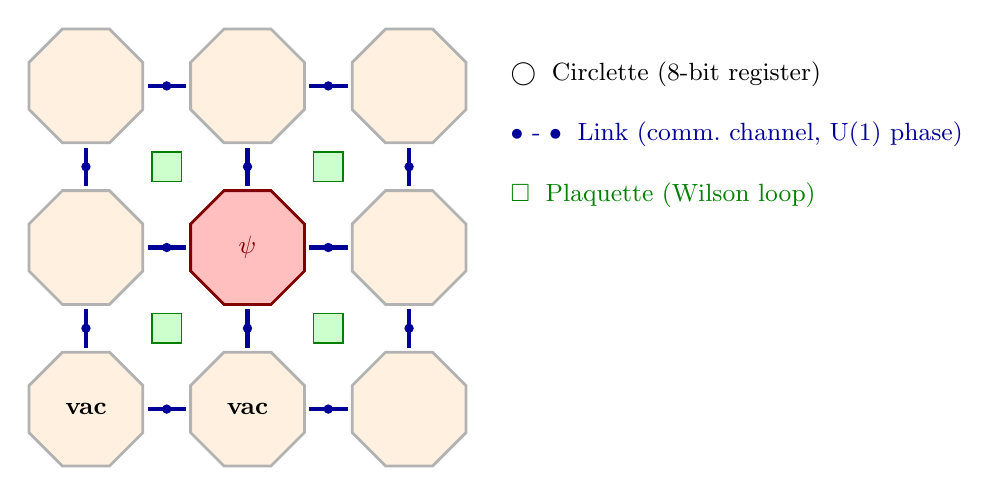
\begin{tikzpicture}[scale=0.85]
% 4.8.8 tiling schematic — all coordinates absolute
\pgfmathsetmacro{\d}{2.414}  % octagon spacing = 1 + sqrt(2)
\pgfmathsetmacro{\R}{0.92}   % octagon circumradius

% Helper: draw an octagon at absolute centre (cx, cy)
\newcommand{\octagon}[4]{% cx, cy, fill colour, edge colour
  \pgfmathsetmacro{\cx}{#1}
  \pgfmathsetmacro{\cy}{#2}
  \draw[fill=#3, draw=#4, line width=1pt]
    ({\cx+\R*cos(22.5)},  {\cy+\R*sin(22.5)}) --
    ({\cx+\R*cos(67.5)},  {\cy+\R*sin(67.5)}) --
    ({\cx+\R*cos(112.5)}, {\cy+\R*sin(112.5)}) --
    ({\cx+\R*cos(157.5)}, {\cy+\R*sin(157.5)}) --
    ({\cx+\R*cos(202.5)}, {\cy+\R*sin(202.5)}) --
    ({\cx+\R*cos(247.5)}, {\cy+\R*sin(247.5)}) --
    ({\cx+\R*cos(292.5)}, {\cy+\R*sin(292.5)}) --
    ({\cx+\R*cos(337.5)}, {\cy+\R*sin(337.5)}) -- cycle;
}

% 1. Plaquettes — drawn first (behind everything)
\foreach \i in {0,1} {
  \foreach \j in {0,1} {
    \pgfmathsetmacro{\sqx}{\i*\d + \d/2}
    \pgfmathsetmacro{\sqy}{\j*\d + \d/2}
    \fill[green!20, draw=green!50!black, line width=0.6pt]
      ({\sqx-0.22}, {\sqy-0.22}) rectangle ({\sqx+0.22}, {\sqy+0.22});
  }
}

% 2. Links — between adjacent octagons
\foreach \i in {0,1,2} {
  \foreach \j in {0,1,2} {
    \pgfmathsetmacro{\ox}{\i*\d}
    \pgfmathsetmacro{\oy}{\j*\d}
    % Horizontal link to right neighbour
    \ifnum\i<2
      \pgfmathsetmacro{\nx}{(\i+1)*\d}
      \pgfmathsetmacro{\lmx}{(\ox+\nx)/2}
      \draw[blue!60!black, line width=1.5pt] ({\ox+\R}, {\oy}) -- ({\nx-\R}, {\oy});
      \fill[blue!60!black] ({\lmx}, {\oy}) circle (2pt);
    \fi
    % Vertical link to upper neighbour
    \ifnum\j<2
      \pgfmathsetmacro{\ny}{(\j+1)*\d}
      \pgfmathsetmacro{\lmy}{(\oy+\ny)/2}
      \draw[blue!60!black, line width=1.5pt] ({\ox}, {\oy+\R}) -- ({\ox}, {\ny-\R});
      \fill[blue!60!black] ({\ox}, {\lmy}) circle (2pt);
    \fi
  }
}

% 3. Octagons — drawn last (on top)
\foreach \i in {0,1,2} {
  \foreach \j in {0,1,2} {
    \pgfmathsetmacro{\ox}{\i*\d}
    \pgfmathsetmacro{\oy}{\j*\d}
    \pgfmathtruncatemacro{\iscentre}{(\i==1 && \j==1) ? 1 : 0}
    \ifnum\iscentre=1
      \octagon{\ox}{\oy}{red!25}{red!50!black}
    \else
      \octagon{\ox}{\oy}{orange!12}{gray!60}
    \fi
  }
}

% 4. Text labels
\node[font=\small\bfseries] at (0, 0) {vac};
\node[font=\small\bfseries] at (\d, 0) {vac};
\node[font=\small\bfseries, text=red!50!black] at (\d, \d) {$\psi$};

% 5. Legend
\node[anchor=west, font=\small] at (6.2, 5.0) {$\bigcirc$\; Circlette (8-bit register)};
\node[anchor=west, font=\small, blue!60!black] at (6.2, 4.1) {$\bullet$ - $\bullet$\; Link (comm.\ channel, $\UU(1)$ phase)};
\node[anchor=west, font=\small, green!50!black] at (6.2, 3.2) {$\square$\; Plaquette (Wilson loop)};

\end{tikzpicture}
\caption{Schematic of the \circlette\ lattice as a 4.8.8 adjacency graph. Octagons are self-contained 8-bit registers; edges are communication channels carrying the gauge phase $U(x,y)$; interstitial squares are plaquettes whose accumulated phase gives the field strength. This is a logical wiring diagram, not a spatial geometry.}
\label{fig:488}
\end{figure}

\emph{Crucially, this diagram is a visual metaphor for the topological adjacency structure, not a literal geometric object.} When two octagons ``share an edge'' in the picture, two \circlettes\ have a communication channel between them. Nothing is shared; nothing overlaps. Each \circlette\ owns its 8 bits absolutely. The edges represent channels through which bits can be read or modified during a tick.

\subsection{The Bandwidth-Matching Principle}
\label{sec:bandwidth}

Each octagon in the 4.8.8 tiling has exactly 8 edges - the same as the number of bits in the \circlette. This numerical coincidence suggests a deeper principle.

On the 4.8.8 graph, each node connects to 8 independent communication channels. These partition into two geometric sectors:

\begin{enumerate}[nosep]
\item \textbf{4 orthogonal channels} connecting to nearest-neighbour octagons (N, S, E, W). These carry the Dirac kinetic term - the spatial hops.
\item \textbf{4 diagonal channels} connecting through interstitial squares to next-nearest-neighbour octagons (NE, NW, SE, SW). These provide the gauge plaquette structure.
\end{enumerate}

The total channel count is:
\begin{equation}
  n_{\text{channels}} = 4_{\text{kinematic}} + 4_{\text{gauge}} = 8 = n_{\text{bits}}.
\label{eq:bandwidth}
\end{equation}

We propose this as a \textbf{bandwidth-matching principle}: an 8-bit register managing 8 independent I/O channels achieves perfect matching between local processing capacity and routing bandwidth. With $n = 7$ bits, the register would lack sufficient internal states for the routing; with $n = 9$, it would have ``dark'' degrees of freedom disconnected from the spatial topology.

\begin{conjecture}[Bandwidth Matching]
The 4.8.8 truncated square tiling is the unique Archimedean tiling of the plane for which the polygon coordination number equals the minimum code length required to support the Standard Model fermion spectrum.
\end{conjecture}


\subsection{Orthogonal Gauge Separation}

On a standard square lattice (tiling 4.4.4.4), the kinematic hops and gauge plaquettes share the \emph{same} edges. On the 4.8.8 lattice, they are topologically distinct: fermion hops use octagon-to-octagon edges, while gauge loops traverse the interstitial square boundaries. This provides a natural separation of data from forces - analogous to the separation of data bus from control bus in computer architecture.

For the CNOT update to evaluate both the spatial hop and the gauge phase within a single clock tick without channel conflict, this separation may be essential: the hop and the phase evaluation cannot simultaneously use the same channel. We formalise this as:

\begin{conjecture}[Single-Tick Consistency]
The 4.8.8 topology is the minimal planar graph that permits both the CNOT kinematic update and the $\UU(1)$ gauge evaluation within a single computational tick without channel conflict.
\end{conjecture}


% ############################################################
\section{Correspondence with Lattice Gauge Theory}
\label{sec:LGT}
% ############################################################

\subsection{Kogut-Susskind Architecture}

The \circlette\ lattice maps directly onto the Kogut-Susskind formulation of Hamiltonian lattice gauge theory~\citep{KogutSusskind1975}:

\begin{center}
\begin{tabular}{lll}
\toprule
\textbf{LGT concept} & \textbf{Circlette realisation} & \textbf{4.8.8 element} \\
\midrule
Site (matter field) & 8-bit register, 45-state code & Octagon \\
Link (gauge field) & $\UU(1)$ phase $U(x,y) = e^{ieA\Delta x}$ & Octagon--octagon edge \\
Plaquette (field strength) & Wilson loop $\prod_\square U$ & Interstitial square \\
Hopping term & CNOT quantum walk & NN channel \\
Wilson mass & CNOT coin operator (dynamical) & N/A (built into dynamics) \\
\bottomrule
\end{tabular}
\end{center}

\subsection{Wilson Loops and Plaquettes}

The interstitial squares of the 4.8.8 tiling are 4-cycles (closed loops of 4 communication links). In lattice gauge theory, the phase accumulated around the shortest closed loop is the \emph{plaquette variable}:
\begin{equation}
  U_\square = U_{12} U_{23} U_{34} U_{41},
\end{equation}
which gives the discretised field strength tensor $F_{\mu\nu}$ in the continuum limit~\citep{Wilson1974}. The 4.8.8 topology natively provides these minimal Wilson loops as geometric features of the tiling.

\subsection{Anomaly Structure from the Code}

As shown in Part~I, the 45-state code automatically satisfies:
\begin{align}
  \sum_f Q_f &= 0 \quad \text{(gravitational anomaly cancellation)}, \\
  \sum_f Q_f^2 &= 16 \quad \text{(exact Standard Model $\beta$-function coefficient)}.
\end{align}
These are \emph{derived} from the constraint structure R1--R4, not imposed.


% ############################################################
\section{The Fermion Doubling Problem}
\label{sec:doubling}
% ############################################################

\subsection{Background: the Nielsen-Ninomiya Theorem}

The Nielsen-Ninomiya no-go theorem~\citep{NielsenNinomiya1981a,NielsenNinomiya1981b} states that on any regular lattice, a Dirac operator satisfying:
\begin{enumerate}[nosep]
\item locality (finite-range hopping),
\item translational invariance,
\item Hermiticity, and
\item exact continuous $\UU(1)_A$ chiral symmetry
\end{enumerate}
necessarily has an equal number of left-handed and right-handed fermion species. In 2D, this produces 4 Dirac points (1 physical, 3 doublers) at the corners of the Brillouin zone.

The standard remedy is the \textbf{Wilson mass}~\citep{Wilson1977}: a momentum-dependent term $M(\mathbf{k}) = r(2 - \cos k_x - \cos k_y)$ proportional to $\beta$ that gaps the doublers while leaving the physical fermion massless. This is added \emph{by hand} and explicitly breaks chiral symmetry.

\subsection{The Dirac Operator on the 4.8.8 Graph}

In the \circlette\ framework, the coin space is spanned by the chirality bit $\chi$ and isospin bit $I_3$, giving 4-component spinors. The Dirac matrices are (Part~I, \S VII):
\begin{equation}
  \alpha_1 = \sigma_x^\chi \otimes \sigma_x^{I_3}, \quad
  \alpha_2 = \sigma_x^\chi \otimes \sigma_y^{I_3}, \quad
  \beta = \sigma_z^\chi \otimes I^{I_3}.
\label{eq:dirac}
\end{equation}
These satisfy the Clifford algebra $\text{Cl}(2,1)$: $\{\alpha_i, \alpha_j\} = 2\delta_{ij}$, $\{\alpha_i, \beta\} = 0$.

On the square lattice with nearest-neighbour (NN) hopping only, the Bloch Hamiltonian is:
\begin{equation}
  H_{\text{naive}}(\mathbf{k}) = \alpha_1 \sin k_x + \alpha_2 \sin k_y,
\label{eq:Hnaive}
\end{equation}
which has zeros at $(0,0)$, $(\pi,0)$, $(0,\pi)$, and $(\pi,\pi)$ - the standard doubling problem.

\subsection{The Geometric Temptation: NNN Hopping}

The 4.8.8 topology provides next-nearest-neighbour (NNN) connections through the interstitial squares. A natural hypothesis is that these diagonal channels act as a \emph{native Wilson mass}, gapping the doublers without any ad-hoc addition.

To test this, we derive the NNN coupling matrix from the two-hop process. A diagonal hop from octagon A to octagon B via an interstitial square involves two consecutive spatial hops:

\begin{center}
\begin{tabular}{lccc}
\toprule
\textbf{Direction} & \textbf{Step 1} & \textbf{Step 2} & \textbf{Combined} \\
\midrule
NE & $\alpha_1$ & $\alpha_2$ & $\alpha_2\alpha_1 = -\alpha_1\alpha_2$ \\
NW & $-\alpha_1$ & $\alpha_2$ & $+\alpha_1\alpha_2$ \\
SE & $\alpha_1$ & $-\alpha_2$ & $+\alpha_1\alpha_2$ \\
SW & $-\alpha_1$ & $-\alpha_2$ & $-\alpha_1\alpha_2$ \\
\bottomrule
\end{tabular}
\end{center}

Summing with Bloch phases $e^{i(\pm k_x \pm k_y)}$:
\begin{align}
  H_{\text{NNN}}(\mathbf{k}) &= t_2 \bigl[
    -\alpha_1\alpha_2\, e^{i(k_x+k_y)} + \alpha_1\alpha_2\, e^{i(-k_x+k_y)} \nonumber\\
    &\qquad + \alpha_1\alpha_2\, e^{i(k_x-k_y)} - \alpha_1\alpha_2\, e^{i(-k_x-k_y)}
  \bigr] \nonumber\\
  &= 4t_2 \sin k_x \sin k_y \cdot \alpha_1\alpha_2.
\label{eq:HNNN}
\end{align}

The product matrix is:
\begin{equation}
  \alpha_1\alpha_2 = (\sigma_x \otimes \sigma_x)(\sigma_x \otimes \sigma_y)
  = I \otimes (i\sigma_z) = i(I^\chi \otimes \sigma_z^{I_3}).
\label{eq:alpha12}
\end{equation}

This is a rotation in the \emph{isospin} sector, \textbf{not} the mass matrix $\beta = \sigma_z^\chi \otimes I^{I_3}$ which acts on \emph{chirality}. The distinction is fundamental: a Wilson mass requires coupling to $\beta$ (chirality mixing); the physical NNN term couples to $\alpha_1\alpha_2$ (isospin rotation).

\subsection{The Rigorous Disproof}
\label{sec:disproof}

The full 4.8.8 Bloch Hamiltonian is:
\begin{equation}
  H_{4.8.8}(\mathbf{k}) = \underbrace{\alpha_1 \sin k_x + \alpha_2 \sin k_y}_{\text{NN (Dirac)}}
  + \underbrace{4t_2 \sin k_x \sin k_y \;\alpha_1\alpha_2}_{\text{NNN (diagonal)}}.
\label{eq:H488}
\end{equation}

At the doubler locations:
\begin{align}
  H_{4.8.8}(\pi, 0) &: \quad \sin\pi \cdot \sin 0 = 0 \quad \Rightarrow \quad \text{NNN term vanishes}, \\
  H_{4.8.8}(0, \pi) &: \quad \sin 0 \cdot \sin\pi = 0 \quad \Rightarrow \quad \text{NNN term vanishes}, \\
  H_{4.8.8}(\pi, \pi) &: \quad \sin\pi \cdot \sin\pi = 0 \quad \Rightarrow \quad \text{NNN term vanishes}.
\end{align}

\begin{result}
The physical NNN coupling generated by the 4.8.8 topology vanishes at all three doubler locations. The 4.8.8 geometry alone \emph{cannot} resolve the fermion doubling problem, regardless of the NNN coupling strength $t_2$.
\end{result}

This result is confirmed by numerical diagonalisation of $H_{4.8.8}(\mathbf{k})$ across the full Brillouin zone for $t_2 \in \{0, 0.1, 0.25, 0.5, 1.0\}$. In all cases, 4 Dirac points persist at the same locations as the naive lattice. The NNN term warps the dispersion relation away from the high-symmetry points but leaves the zeros untouched. See the companion numerical code~\citep{FermionDoublingCode}.

Furthermore, we exhaustively tested all possible NNN coupling matrices $\Gamma \in \{I, \beta, \alpha_1, \alpha_2, i\alpha_1\alpha_2, \alpha_1\beta, \alpha_2\beta\}$ with a Wilson-like $\cos k_x \cos k_y$ dependence. While the $(\pi,0)$ and $(0,\pi)$ doublers \emph{can} be gapped by a term $\Gamma \cdot (1 - \cos k_x \cos k_y)$, the $(\pi,\pi)$ doubler \emph{cannot}: $\cos\pi\cos\pi = 1 = \cos 0 \cos 0$, so the mass at $(\pi,\pi)$ always equals the mass at $(0,0)$. The NNN structure of the 4.8.8 graph, regardless of coupling matrix, cannot distinguish the physical fermion from the $(\pi,\pi)$ doubler.


\subsection{The Algorithmic Resolution: the CNOT Coin}
\label{sec:CNOT}

The resolution comes not from the spatial topology but from the \emph{dynamics}.

In the theory of discrete-time quantum walks (DTQWs), as established in the quantum cellular automaton frameworks of D'Ariano and Perinotti~\citep{DAriano2014,Bisio2015,Venegas2012}, the coin operator - the internal-state update applied at each tick before the conditional shift - is the sole generator of the effective mass in the continuum limit. In the \circlette\ framework, the coin operator is the \textbf{CNOT gate}:
\begin{equation}
  \text{CNOT}: \quad \chi \to \chi, \quad W \to W \oplus \chi.
\end{equation}
This copies the chirality bit $\chi$ into the weak bit $W$, enforcing the R2 constraint $\chi \oplus W = 0$ at each tick. In the language of quantum field theory, this is an \emph{explicit, dynamical mixing of the left-handed and right-handed chiral sectors} at every computational step.

The Nielsen-Ninomiya theorem~\citep{NielsenNinomiya1981a,NielsenNinomiya1981b} is fundamentally a topological winding theorem: it requires that the \emph{continuous} phase $\UU(1)_A$ accumulated around the Brillouin zone torus sums to zero, mandating equal numbers of left- and right-handed species. But in the \circlette\ framework:

\begin{enumerate}[nosep]
\item Chirality is a \textbf{discrete Boolean variable} $\chi \in \{0, 1\}$, not a continuous phase.
\item The ``chiral symmetry'' is $\ZZ_2$ (bit flip), not $\UU(1)_A$ (continuous rotation).
\item A discrete binary state space does not support the topological winding required by the theorem. Formally, the fundamental group $\pi_1(\UU(1)) = \ZZ$ permits integer winding numbers across the Brillouin zone torus, which is the mechanism that mandates doublers. A discrete $\ZZ_2$ space has no continuous manifold; topological winding is strictly undefined, and the homotopy prerequisites for the theorem are entirely absent.
\end{enumerate}

\begin{result}
The Nielsen-Ninomiya theorem is inapplicable to the \circlette\ lattice because its foundational premise - exact continuous $\UU(1)_A$ chiral symmetry - is violated by the discrete $\ZZ_2$ structure of the chirality bit and its CNOT update rule.
\end{result}

The CNOT coin serves the same mathematical function as the Wilson mass term: it couples the two chirality sectors with a strength that depends on the lattice momentum. But unlike the Wilson mass, which is an ad-hoc dimension-5 operator bolted onto the action, the CNOT is the \emph{fundamental computational engine of time} - the tick-level update that defines the quantum walk. The doublers are not gapped by a penalty term; they simply never arise, because the symmetry that would protect them does not exist in the discrete theory.

This distinction is summarised in Table~\ref{tab:comparison}.

\begin{table}[H]
\centering
\caption{Comparison of doubler resolution mechanisms.}
\label{tab:comparison}
\begin{tabular}{lcc}
\toprule
& \textbf{Wilson fermions} & \textbf{Circlette (CNOT coin)} \\
\midrule
Chiral symmetry & $\UU(1)_A$ broken explicitly & $\ZZ_2$ (never continuous) \\
Mechanism & Momentum-dependent mass & Discrete chiral mixing \\
Origin & Added by hand & Fundamental dynamics \\
Level & Hamiltonian (spatial) & Coin operator (temporal) \\
Nielsen-Ninomiya & Evaded (symmetry broken) & \textbf{Inapplicable} (wrong axiom) \\
Physical mass & From Wilson parameter $r$ & From CNOT frequency \\
\bottomrule
\end{tabular}
\end{table}


% ############################################################
\section{Hardware and Software: A Separation of Concerns}
\label{sec:discussion}
% ############################################################

\subsection{The Architecture}

The results of Sections~\ref{sec:488} and \ref{sec:doubling} establish a clean decoupling:

\paragraph{Hardware (the 4.8.8 topology):}
\begin{itemize}[nosep]
\item Establishes the $n = 8$ bandwidth matching (code length = coordination capacity).
\item Separates kinematic channels from gauge channels (orthogonal gauge separation).
\item Provides native Wilson-loop plaquettes as interstitial squares.
\item Defines the spatial adjacency structure from which distances emerge.
\end{itemize}

\paragraph{Software (the CNOT dynamics):}
\begin{itemize}[nosep]
\item Generates the Dirac equation as the continuum limit of the quantum walk.
\item Provides dynamical chiral mixing, resolving fermion doubling.
\item Produces rest mass as the CNOT execution frequency.
\item Enforces the R1--R4 constraints that define the particle spectrum.
\end{itemize}

The hardware is the routing network; the software is the physics. This is not a metaphor - it is a precise architectural statement. The spatial topology determines \emph{who can talk to whom}; the update rule determines \emph{what they say}.

\subsection{Distance and Geometry}

In the background-independent picture, distance between two \circlettes\ is the number of hops (graph distance). The link variables $U(x,y)$ modulate this: regions with large phase fluctuations have shorter effective distances (information propagates more easily). The metric tensor emerges from the Fisher information geometry of the link variables, as shown in Part~I. Curved spacetime is a region where the link variables vary systematically; a gravitational well is a region where more hops fit into a given coordinate distance.

\subsection{What Position Means}

A particle ``at position $x$'' means: the wavefunction amplitudes are concentrated around the nodes in the neighbourhood of $x$, where $x$ is defined by its graph relationships to everything else. The question ``where is the electron?'' asks ``at which nodes are the \circlette\ states carrying non-negligible amplitude for an electron-type codeword?'' Position is not a property of the lattice - it is a statement about the distribution of information \emph{on} the lattice.


% ############################################################
\section{Open Questions}
\label{sec:open}
% ############################################################

\subsection{Is the 4.8.8 Tiling Unique?}

The bandwidth-matching argument (Conjecture~1) is currently a heuristic. A proof would require showing that:
\begin{enumerate}[nosep]
\item The 4.8.8 tiling is the unique Archimedean tiling with coordination number 8 and bipartite gauge structure.
\item No other tiling can support the 45-state fermion spectrum with anomaly cancellation.
\end{enumerate}

This is a well-posed mathematical question amenable to exhaustive enumeration of Archimedean tilings (there are only 11).

\subsection{Can the CNOT Resolution Be Made Rigorous?}

We have argued that the Nielsen-Ninomiya theorem is inapplicable because the \circlette's chirality is $\ZZ_2$ rather than $\UU(1)_A$. A rigorous proof would require:
\begin{enumerate}[nosep]
\item Explicit construction of the DTQW propagator with the CNOT coin.
\item Computation of the effective continuum Lagrangian and demonstration that no doubler poles appear in the fermion propagator.
\item Verification that the $\ZZ_2$ symmetry is sufficient for anomaly cancellation but insufficient for topological winding.
\end{enumerate}

This connects to the broader programme of deriving quantum field theory from quantum cellular automata~\citep{DAriano2014,Bisio2015,BialynickiBirula1994}.

\subsection{The Brillouin Zone Folding Question}

The bipartite structure of the 4.8.8 tiling (two sublattice types for the interstitial squares) doubles the real-space unit cell and halves the Brillouin zone. The reciprocal lattice vector $\mathbf{b}_1 = (\pi, \pi)$ maps the $(\pi,\pi)$ doubler onto the physical $(0,0)$ point. Whether this folding \emph{absorbs} the final doubler into the internal spinor degrees of freedom (as in Kogut-Susskind staggered fermions~\citep{KogutSusskind1975}) or merely \emph{aliases} it remains an open question requiring explicit computation of the folded Hilbert space.


% ############################################################
\section{Conclusions}
\label{sec:conclusions}
% ############################################################

We have established the ontological and topological foundations of the \circlette\ lattice:

\begin{enumerate}
\item The \circlettes\ \emph{are} the lattice (background independence). Spacetime is an emergent property of informational adjacency. Particles are information gliders on a fully occupied vacuum substrate.

\item The 4.8.8 truncated square tiling provides the natural topological graph, with a structural coincidence $n_{\text{bits}} = n_{\text{channels}} = 8$ suggesting a bandwidth-matching principle.

\item The correspondence with Kogut-Susskind lattice gauge theory is exact: octagons are sites, edges are links, interstitial squares are plaquettes.

\item The 4.8.8 NNN coupling generates a term proportional to $\alpha_1\alpha_2 \times \sin k_x \sin k_y$, which \emph{vanishes at all doubler locations} and cannot resolve fermion doubling. This was rigorously verified by explicit matrix algebra and numerical Brillouin zone scanning.

\item The fermion doubling problem is resolved at a deeper level: the CNOT coin operator's discrete $\ZZ_2$ chiral mixing makes the Nielsen-Ninomiya theorem inapplicable. The doublers are not gapped - they never arise.

\item The separation of concerns between hardware (topology) and software (dynamics) provides a clean architectural foundation for the ``It from Bit'' programme.
\end{enumerate}

While the structural alignment between the 8-bit \circlette\ capacity and the 8-channel routing of the 4.8.8 adjacency graph cleanly resolves theoretical bottlenecks, we propose it here as a heuristic. Whether the 4.8.8 topology is the unique planar graph mathematically required to support the fermion spectrum and $\UU(1)$ gauge structure - and whether the CNOT resolution of fermion doubling can be elevated to a theorem - remain compelling open questions for subsequent investigation.


% ############################################################
% REFERENCES
% ############################################################

\bibliographystyle{unsrtnat}
\bibliography{circlette-lattice-refs}

\end{document}
